%
% File acl2015.tex
%
% Contact: car@ir.hit.edu.cn, gdzhou@suda.edu.cn
%%
%% Based on the style files for ACL-2014, which were, in turn,
%% Based on the style files for ACL-2013, which were, in turn,
%% Based on the style files for ACL-2012, which were, in turn,
%% based on the style files for ACL-2011, which were, in turn, 
%% based on the style files for ACL-2010, which were, in turn, 
%% based on the style files for ACL-IJCNLP-2009, which were, in turn,
%% based on the style files for EACL-2009 and IJCNLP-2008...

%% Based on the style files for EACL 2006 by 
%%e.agirre@ehu.es or Sergi.Balari@uab.es
%% and that of ACL 08 by Joakim Nivre and Noah Smith

\documentclass[11pt]{article}
\usepackage{acl2015}
\usepackage{times}
\usepackage{url}
\usepackage{latexsym}
\usepackage{amsopn}

%%%%%%%%%%%%%%%%%%%%%%%%%%%%%%%%%%%%%%%%%%%%%%%%%%%%%%%%%%%%%%%%%%%%
%% KUI'S STANDARD PREAMBLE
%%%%%%%%%%%%%%%%%%%%%%%%%%%%%%%%%%%%%%%%%%%%%%%%%%%%%%%%%%%%%%%%%%%%

\usepackage{subfigure}
\usepackage{algorithm}
\usepackage{algorithmicx}
\usepackage{algpseudocode}
\usepackage{xcolor}
\usepackage{tabularx}

\usepackage{graphicx}
\DeclareMathOperator{\conv}{conv}
\DeclareMathOperator{\st}{s.t.}
\DeclareMathOperator{\dom}{dom}
\DeclareMathOperator{\im}{im}
\DeclareMathOperator{\Ne}{Ne}
\DeclareMathOperator{\sign}{sign}
\DeclareMathOperator{\Var}{Var}
\DeclareMathOperator{\diag}{diag}
\DeclareMathOperator{\vvec}{vec}


%\setlength\titlebox{5cm}

% You can expand the titlebox if you need extra space
% to show all the authors. Please do not make the titlebox
% smaller than 5cm (the original size); we will check this
% in the camera-ready version and ask you to change it back.

\title{Topic Models for Texts and Images in Representation Space}

\author{Kui Tang \\
  Columbia University \\
  {\tt kt2384@columbia.edu} \\\And
  Sameer Lal \\
  Columbia University \\
  {\tt sl3368@columbia.edu} \\}
%\date{10 May 2015}
\date{}

\begin{document}
\maketitle

\begin{abstract}
Recent work has shown promising results in obtaining low-dimensional semantic embeddings of discrete (text) or high-dimensional (image) data. So far, these embeddings have only been applied to fine-grained discriminative tasks such as image captioning or analogy completion. Embedding such vectors in higher order statistical models is an open problem with applications to information retrieval, document summarization, recommendations, and other areas. This work proposes a novel topic model to work in this multimodal space where all document elements (words and images) are represented as word vectors. Vectors are clustered into a mixture of Gaussians, each representing a latent ``concept.'' Topics are latent mixtures of Gaussians, and each document is a mixture of topics. Pre-trained state-of-the-art neural networks are used to obtain feature mappings for words and images. A linear mapping between image and word vectors are learned to put all data into the same space. We present qualitative and quantitative results showing improvement against baseline LDA and conclude and propose future work.
\end{abstract}

\section{Introduction}
One of the popular tasks in Machine Learning and Computer Vision has been object detection. The ability for computers to recognize patterns in image data has many applications in robotics, health care, manufacturing, and defense. For many years, traditional computer vision algorithms were capable of achieving mediocre performance in object recogntion challenges. Recently though, the use of convolutional neural networks has led researchers to achieve significantly higher levels of performance. This breakthrough has been met with a rapid adoption of deep learning in many other domains. Neural nets have been used in natural language processing, speech recognition, facial detection, and reinforcement learning. Having developed a powerful tool for supervised learning across multiple modalities of data, a new challenge arises in performing learning in this multimodal space. Given the ability to extract rich features via neural networks and the abundance of unsupervised multimodal data, research focus has shifted to building models which could learn semantic information from these natural data sets such as news articles or annotated images. By extracting features from this space, statistical models could gain a much deeper understanding of objects and concepts. 

\section{Related Work}
\paragraph{Neural multimodal models.}
\cite{Lecun98} propose joining several neural network models for multimodal learning into a joint objective function, and then optimizing the parameters of each to maximize performance on this joint measure. \cite{Srivastava14} propose a joint text-image model using RBMs. Their model is fully generative, and the textual model is an undirected analogue to a topic model. However, they are unable to leverage state-of-the-art CNN image features, and they rely on contrastive divergence for learning, which limits scalability. They also rely on a binary semantic space, while ours is real.

\paragraph{Topic models on shallow image features.}
Several authors have applied topic modeling to visual or joint text and visual data, but none to date have utilized deep semantic representations as image features. \cite{Barnard03} considers several models beginning with marginally independent emission distributions for words and image blobs (which are nevertheless conditional dependent) and proceeds to model additional dependencies between the distributions. \cite{Wang09a} model alignment between words and image patches, but train on a supervised dataset and use only bag of codeword features to represent images, with codewords generated by $k$-means and SIFT. Moreover, these methods are designed only for supervised image captioning.

Some work has used topic models in unsupervised settings for images. \cite{Fritz08} trains LDA to detect object categories, but they use only gradient histogram representations. \cite{Cao07} proposed a model for unsupervised object detection, but they only used quantized SIFT features.

\paragraph{Hybrid neural network and HMM models.}
A simpler problem related to our work is to combine output from a feedforward neural network with a Hidden Markov model. Several authors have proposed schemes tuned for a variety of tasks \cite{Trentin01}. The approach closest to ours is that of \cite{Bengio92}, which derives gradient updates to a feedforward neural network based on the maximum-likelihood objective. Our work shares the same approach to optimize the neural network parameters to maximize the likelihood of the overall probabilistic model.

\section{Models}
\begin{figure}
\centering
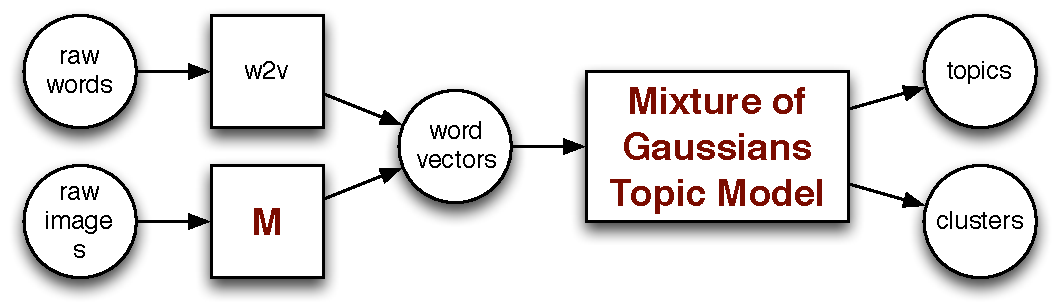
\includegraphics[width=\columnwidth]{assets/stagewise_model.pdf}
\caption{\label{fig:stagewise} Diagram of stagewise multimodal model of this work. Black boxes denote standard pretrained models. Round entries are intermediate representations, and green boxes denote components we trained.}
\end{figure}

Figure~\ref{fig:stagewise} outlines the model presented in this work, which can be viewed as a stagewise approximation to a fully Bayesian treatment of the problem. We first obtain pre-trained models which take words or images as inputs and output rich continuous features representations (details in Sec.~\ref{:sec:data}). We replicate the approach in \cite{Frome13} to learna linear map to transform image vectors to word vectors by minizing a ranking loss

$$\ell(v, y) = \sum_{y' \neq y} \max \left[0, \lambda - w_{y}^\top M v + w_{y'} ^\top M v \right]$$

where $v$ is image vector, $y$ is image label, $w$ is word vector. Sum this term over all $(v, y)$ pairs in labeled data. Instead of summing all $y' \neq y$, we randomly iterate over $y'$ and return first example violating the margin.

Having obtained a trained $M$ matrix, we now take each image in our corpus and run it through the image model (AlexNet) and multiply it by $M$ to obtain a transformed word vector for that image.

Now that all components of the data have been transformed to a common feature representation (word vectors), we are ready to fit the mixture of Gaussians topic model.

\subsection{Mixture of Gaussians Topic Model}
The model assumes a large dictionary of ``concepts'', which are Gaussian clusters in semantic space. A topic is a mixture of these concepts, and each vector $x_{dn}$ (word or image) is described by a mixture of topics. The generative process is as follows:

\begin{itemize}
\item For $k = 1, \ldots, K$ (for each topic):
  \begin{itemize}
    \item Draw $\beta_k \sim \mbox{Dir}(\alpha=10^{-6})$
    \item Draw $\lambda_k \sim \mbox{Gamma}(10^{-6}, 10^{-6})$
    \item Draw $\mu_k \sim \mathcal{N}(0, \diag(\tau))$
  \end{itemize}
\item For $d = 1, \ldots, D$ (for each document):
  \item Draw $\theta_d \sim \mbox{Dir}(\gamma)$
  \item For $n = 1, \ldots, N_d$ (for each word in document):
  \begin{itemize}
    \item Draw $z_{dn} \sim \mbox{Mult}(\theta_{dn})$
    \item Draw $c_{dn} \sim \mbox{Mult}(\beta_{z_{dn}})$
    \item Draw $x_{dn} \sim \mathcal{N}(\mu_{c_{dn}}, \diag(\tau_{c_{dn}})$
  \end{itemize}
\end{itemize}

As this model is conjugate-exponential family we perform posterior inference using variational message passing (VMP)~\cite{Winn05} using the BayesPy package~\cite{Luttinen14}.

We attempted to implement stochastic variational inference~\cite{Hoffman13} for this model, but were unable to converge to high-quality local optima. We hypothesize this is due to model mis-specification (details deferred to Sec.~\ref{sec:misspec}). In short, mixture models benefit from asymmetric initializations, particularly when we seek sparse posteriors (as in this case, where we want topics to put zero probability mass on most concepts). However, our mis-specified likelihood results in numerical underflow for asymmetric initializations. The batch VMP algorithm is able to overcome a symmetric initialization, but not so the stochastic algorithms.

\section{Results}
\begin{figure}
\centering
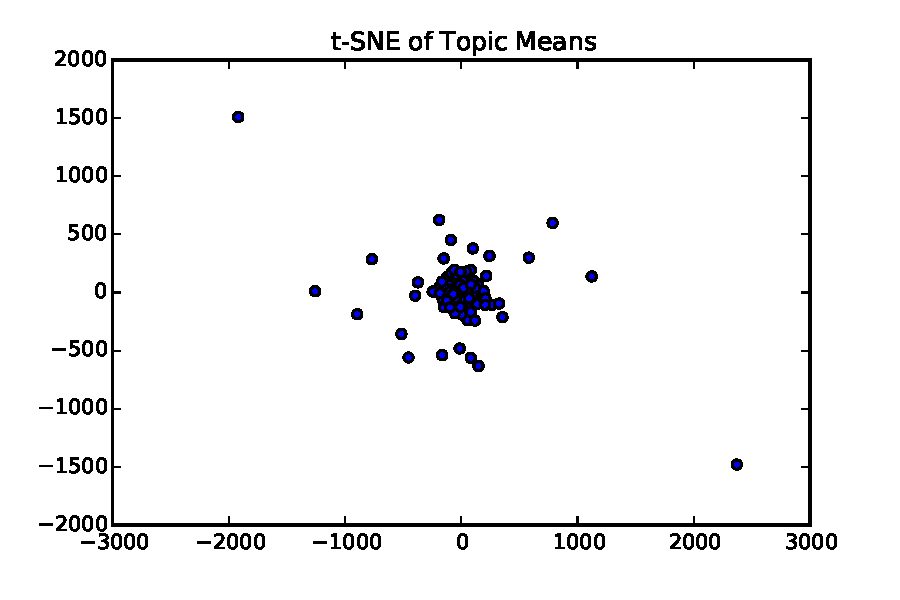
\includegraphics[width=\columnwidth]{assets/gtm100_mu_tsne.pdf}
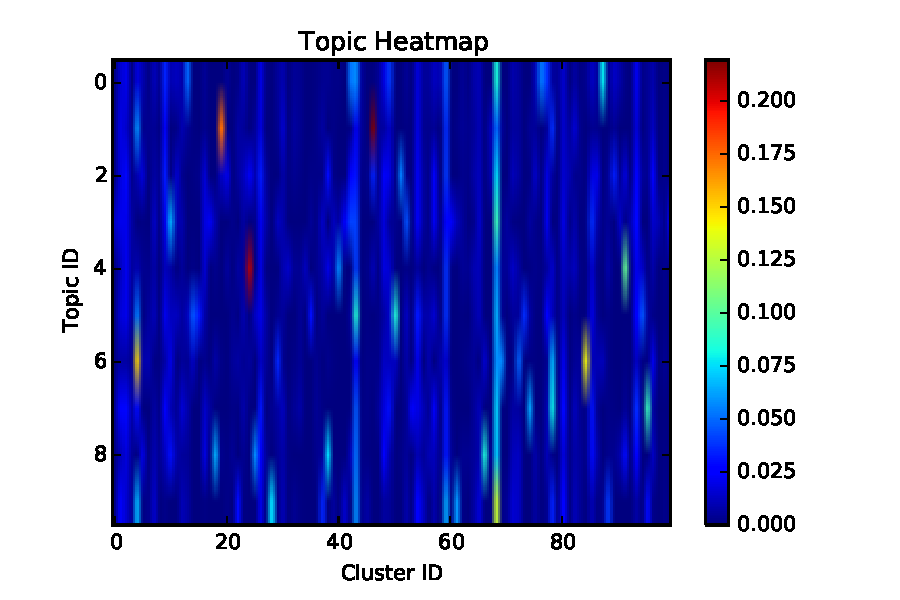
\includegraphics[width=\columnwidth]{assets/gtm100_topic_heatmap.pdf}
\caption{\label{fig:gtm-globals} \emph{Top:} Locations of means of 100 concept clusters ($t$-SNE). \emph{Bottom:} Distribution of topics (rows) over clusters (columns).}
\end{figure}

\begin{figure}
\centering
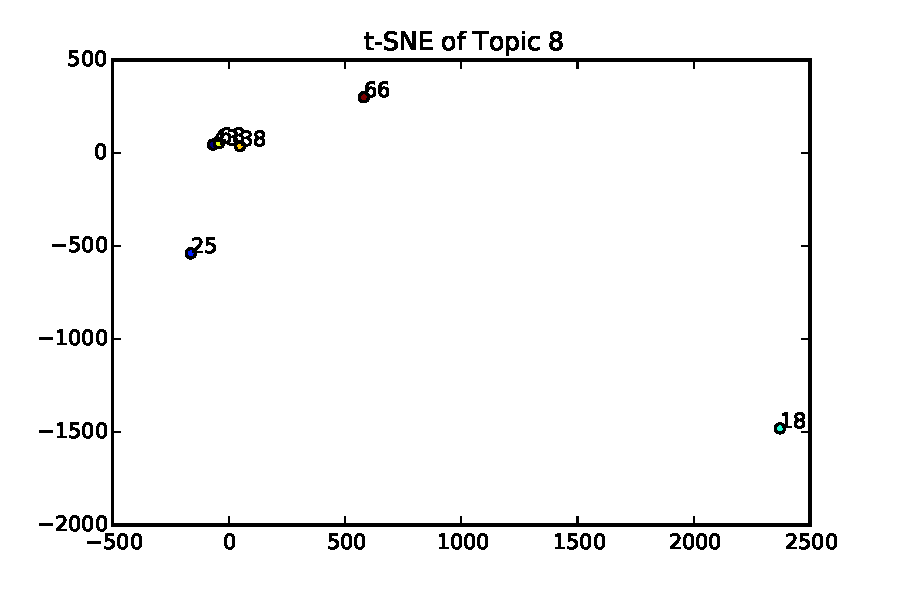
\includegraphics[width=\columnwidth]{assets/gtm100_topic8_tsne.pdf}
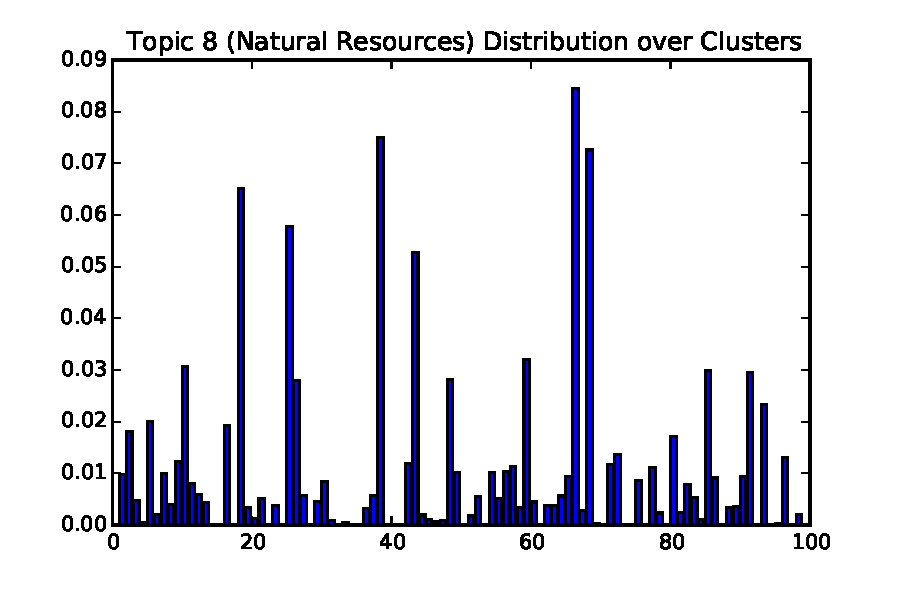
\includegraphics[width=\columnwidth]{assets/gtm100_topic8_probs.pdf}

\begin{tabularx}{\columnwidth}{|c|X|}
\hline 
{\tiny{}Cluster} & {\tiny{}Words}\tabularnewline
\hline 
{\tiny{}18} & {\tiny{}\textbf{[Saltwater]} shoreline ocean coastline nearshore\_reefs sandy\_shorelines
coastal\_waters shallow\_reefs tidal\_creek shallow\_waters mud\_flats
sea tidal\_inlet pier\_pilings underwater reef shoreward abyssal\_plain
inter\_tidal shifting\_sandbars sandy\_bottomed }\tabularnewline
\hline 
{\tiny{}25} & {\tiny{}\textbf{[Freshwater]} water ice surface green porpoise\_vaults surficial\_aquifer
rainwater Floridan\_aquifer radar\_deflectors wa\_ter absorbs\_carbon\_dioxide
bermed absorbs\_sunlight bugs\_wiggling Mosquitoes\_breed overflowing\_septic\_tanks
mild\_dishwashing\_liquid reverse\_osmosis\_filtration hyper\_saline
secondary\_clarifier }\tabularnewline
\hline 
{\tiny{}38} & {\tiny{}\textbf{[Chemicals]} hydrous calcium\_oxide cyclohexane inorganic\_salts calcium\_sulphate
fluorocarbons Sodium\_cyanide silicate\_rocks Nitric\_acid chemically\_reactive
calcium\_carbonates magnesium\_silicate outgas raffinate potassium\_salts
bacterial\_decomposition methane trihalomethanes\_THMs element\_boron
Sulphur\_dioxide }\tabularnewline
\hline 
{\tiny{}66} & {\tiny{}\textbf{[Volcanoes]} coral reefs reef corals coral\_reefs ocean volcanoes sea coral\_reef
volcanic islands lava volcano oceans undersea\_volcanoes oceanic ocean\_basins
lava\_flows eruptions Kilauea\_Volcano}\tabularnewline
\hline 
\end{tabularx}

\caption{\label{fig:gtm-nat-res} \emph{Top:} Locations of means of significant ($\geq 5\%$ posterior probability) concept clusters for the ``natural resources'' topic ($t$-SNE). \emph{Bottom:} Distribution over concept clusters for the ``Natural resources'' topic.}
\end{figure}

\begin{table}
\centering
\begin{tabular}{|c|c|c|}
\cline{2-3} 
\multicolumn{1}{c|}{} & LDA & MoG-LDA\tabularnewline
\hline 
Test log-likelihood & $-11.915$ & $4.7370 \times 10^7$ \tabularnewline
\hline 
Test perplexity & $3860.5$ & \tabularnewline
\hline 
Avg. observed coherence & $0.00509$ & $0.01666$ \tabularnewline
\hline 
Avg. word intrusion & $0.60$ & $0.30$ \tabularnewline
\hline 
\end{tabular}
\caption{\label{fig:quant} Quantitative results comparing mixture of Gaussian LDA (with pretrained word vectors) with ordinary LDA. All log-likelihood and perplexity results were obtained by training on last 100 documents and testing on first 100 as described in Sec.~\ref{sec:data}. The topic coherence metrics are described in \cite{Lau14} using code supplied by the author. Note that test log-likelihood for mixture of Gaussian LDA is positive because it the likelihood is a continuous density, and thus not directly comparable, and also due to mis-specification (see Sec.~\ref{sec:misspec}).}
\end{table}

[WRITE ABOUT HOW WE SELECTED WIKIPEDIA.]

We compare results between LDA~\cite{Blei03} and our method (batch training) trained over the last 100 documents on our Wikipedia dataset, containing 133,866 words. We set both methods to fit 10 topics. Table~\ref{tbl:topics} shows ten most probable words under each topic for each method. Figure~\ref{fig:gtm-globals} summarizes the mixture of Gaussians learned by our model, while Figure~\ref{fig:gtm-nat-res} zooms in on one particular topic (which we label natural resources) to examine four significant clusters within it.

\subsection{Data}
\label{sec:data}
Image vector data was extracted using the popular deep learning image processing library Caffe \cite{Jia14}. The library's pretrained \textit{CaffeNet} convolutional neural network was used to classify images. For each image in the training set of the ILVRC, the output of the final rectified linear unit was recorded. These 4096 dimensional vectors were used in image and word alignment. For word vectors, the first word in each class' synset which existed in the pretrained \textit{word2vec} \cite{Mikolov13a} mapping was used to extract a word vector. The mapping was trained on Google New's corpus of over 10 billion words. To obtain pertinent documents for topic modeling, the raw text of the Wikipedia article for each class' synset was treated as a document. There were several classes that did not have a \textit{word2vec} mapping or valid Wikipedia article and those were simply ommitted. In order to have documents with multimodal information, each word in the Wikipedia articles was transformed into \textit{word2vec} vector. Then each article was appended with 10 images that had been mapped to the word vector space (300 dimensional) using the Image-Word alignment.

\subsection{Quantitative Evaluation}

\subsection{Model Mis-specification:}
\label{sec:misspec}
our pretrained word vectors (obtained from the authors' website of~\cite{Mikolov13a}) were normalized, but the Gaussian likelihood does not generate unit-norm vectors, particularly when the mean is close to an existing word vectors and therefore has norm close to one (as we observe occured). 

\section{Discussion}

\section{Conclusions and Future Work}

\section*{Acknowledgments}

We thank Profs. Liangliang Cao and James Fan for organizing a deep learning course, encouraging us to explore multimodal models, and for their advice on evaluation.

% include your own bib file like this:
\bibliographystyle{acl}
\bibliography{ML}

%\begin{thebibliography}{}
%\end{thebibliography}

\end{document}
